
\begin{refsection}

\newrefcontext[sorting=ynt]

\lettrine{B}{irds} are unique in moving mostly by powered flight on feathered wings.
Feathers, unlike animal hair and claws, are dead proteinaceous structures, which cannot be renewed continuously as they suffer wear and tear \cite{rayner1988,jenni1989}.
As feathers mature, the wing condition and consequently flight capacity of birds gradually decreases \cite{lindstrom1994,hedenstrom1999,hedenstrom2003}.
This makes maintaining wing condition through molt --- the shedding of old, worn-out feathers, and their replacement with freshly grown ones --- a key process in avian ecology \cite{ginn1983,rayner1988}.
During wing molt, as one or more old feathers are lost and new ones grow in their place, the flight surfaces of bird wings become smaller.
The reduction in flight surface area can be measured using a robust-cross species index, which corresponds to the size of the gap in the flight surface during the molt process \citep{lind2001,kiat2016}.
Wider gaps lead to larger (temporary) reductions in wing surface area, power output, and flight capacity and efficiency in captive birds \cite{tucker1991,swaddle1996,swaddle1997,williams2003,lind2001,lind2001a,bowlin2009}.
In addition to these indirect costs, wing molt is among the most energetically demanding phases of a bird's annual cycle, as substantial resources must be channelled towards regrowing large flight feathers \cite{lindstrom1993,newton2009,kiat2017}.
Despite these clear mechanistic links between molt and movement, our understanding of the movement strategies and habitat selection of molting birds in the wild is poor.

The direct influence of wing molt on the movement and habitat preferences of birds has primarily been examined in a few small-scale, disconnected studies \citep{bell1970,haukioja1971,green1975,francis1991,madsen1987,fox1998}.
Moving less, as some northerly species of finches and buntings do \citep{bell1970,haukioja1971,green1975,francis1991}, could save energy required to regrow feathers.
Avoiding predation risk during molt by sheltering in vegetation and rough terrain \citep{bell1970,haukioja1971,green1975,francis1991}, or near water-bodies as geese and ducks do \cite{madsen1987,fox1998}, could also lead to reduced movement during molt.
Molt often co-incides with migratory periods \citep{kiat2019}, making it difficult to separate the effects of migration-related energetic requirements \cite{alerstam1990,wikelski2003,horvitz2014} from molt-related considerations on habitat selection, such as for high-quality resources \cite{madsen1987,fox1998}.
Simultaneously, molt itself is influenced by bird physiology, with large-bodied species molting faster \citep{kiat2021,jenni2020}, and also by birds' movement strategies, as wide-ranging species molt more slowly to maintain movement capacity \cite{kiat2016}.

A robust examination of the direct effects of molt would be to study a set of unrelated, non-migratory species that are not constrained by the short time available for molt in northern temperate regions \cite{ginn1983,jenni2020}.
The cross-species study of movement and habitat selection in molting birds could benefit from dramatic advances in the high-throughput position tracking of small species \cite{toledo2020,nathan2022}, and from the use of standardised data pre-processing and analysis pipelines \cite{gupte2022d}.
Birds, like many animals, can take the spatial perspective of potential threats, such as predators, and avoid risky, exposed areas \cite{hampton1994,emery2000,krams2001,davidson2016}.
Adopting a mechanistic, viewshed ecology approach \cite{olsoy2015,aben2018,aben2021} in habitat selection analyses could account for birds' visibility to potential predators, \cite{olsoy2015,aben2018,aben2021}, while also avoiding confounds with the resource-provisioning effects of sheltering vegetation \citep{pettorelli2011}.

We present a first exploration of the direct effects of wing molt on the movement of birds, focusing on four sympatric, non-migratory, sub-tropical species: House sparrows (\textit{Passer domesticus}), White-spectacled bulbuls (\textit{Pycnonotus xanthopygos}), Clamorous reed warblers (\textit{Acrocephalus stentoreus}), and Barn swallows (\textit{Hirundo rustica}).
We combined molt gap scoring, experimental manipulation of molting birds, high-throughput tracking, and high-resolution viewshed analysis to study how molt affected birds' preferences for sheltered habitats, in the Hula Valley, Israel.
Scoring the molt-related wing gap size \citep{lind2001,kiat2016} of naturally molting and non-molting birds, we manipulated a subset of molting individuals by removing a number of flight feathers.
We tracked birds using the high-throughput ATLAS system \citep{toledo2014,weiser2016,toledo2020}, and examined \textit{(i)} how the size of the molt-related gap affected bird movement, and \textit{(ii)} how the molt gap size influenced selection for more sheltered habitats.
Overall, we show how birds' movement decisions, influenced by their immediate physiological condition, scale up to affect their space use, and how individuals' adaptive strategies have feedbacks with their evolutionary ecology.

\section*{Methods}

We studied bird molt and movement in the Hula Valley of northern Israel (33.10°N, 35.60°E), which includes reconstructed wetlands and reedbeds as well as agricultural areas (crops, plantations and fishponds; see \textit{SI Appendix}).

\subsection{Bird capture and wing molt scoring}

We captured 94 individuals of four species in 2016: 19 White-spectacled bulbuls (\textit{Pycnonotus xanthopygos}), 38 House sparrows (\textit{Passer domesticus}), 16 Clamorous reed warblers (\textit{Acrocephalus stentoreus}), and 21 barn swallows (\textit{Hirundo rustica}).
We caught all individuals before the molting season commenced but after breeding was completed, between June and October 2016.

We first described the state of each primary feather on a scale of 0 to 5 using the primary score (PS) method \citep{ginn1983}.
Both PS = 0 and PS = 5 indicate a fully mature feather, and hence no gap in the wing.
A PS value between 1 and 4 indicates feathers in increasing stages of maturation, with PS = 1 representing a large gap left by a recently molted feather.
This method allows a cross-species estimate of the size of the molt-related gap in the wing, and is also strongly and negatively correlated with molt speed and duration \citep{rohwer2009}.
We scored the wing gap size due to any single feather molting as the inverse value of PS for each of the wing's nine primary feathers (P1 -- P9; counted outward) such that when PS = 1, gap size = 4, and when PS = 2, wing gap size = 3, etc.
However, for PS = 0, wing gap size is also 0 because there is no gap in both the PS = 0 and PS = 5 stages, as either an old, mature feather, or a new, freshly grown feather is present.
To compare molt-related wing gap sizes across individual birds, we summed the wing gap size scores across all nine primary flight feathers, for each individual, into a single wing gap index \citep{kiat2016}.
This index is independent of the size of individual birds and their morphology, controls for the stage of wing feather molt, and allows for reliable cross-species comparisons \citep{bensch1993,kiat2016}.

We experimentally manipulated 29 individuals across species {(bulbuls = 6, sparrows = 14, reed warblers = 2, swallows = 7)}, and removed between one and three primaries, in addition to the primaries missing as part of natural molt.
These primaries were removed by cutting the feather near its base, and this procedure simulates an enlargement of the molt-related wing gap.
Cutting the feather rather than tearing it out from the base, which is still innervated \cite{jenni2020}, avoids excess trauma which could impact birds' behaviour, and allowed us to examine the effect of only the gap size on movement and habitat selection.
For these experimentally manipulated birds, we calculated the wing gap size after the manipulation described here.
Bird capture and handling, the experimental manipulation procedure, and tagging for position tracking (see below) were conducted under a permit from the Israel Nature and Parks Authority (NPA permit 2016/41402) and from the ethics committee of the Hebrew University of Jerusalem, Israel (NS-16-14801-2).

\subsection{Forecasting daily changes in the wing gap size index}

The size of the molt-related wing gap decreases slowly and constantly as feathers regrow, yet as a mature feather is shed, the wing gap size may also increase in gradual jumps.
Over our tracking period of about 7 days per individual (see below), this is expected to represent small changes in the wing surface area, which could further influence movement decisions.
These changes in wing condition should be accounted for when relating movement characteristics to wing gap size.
To do this, we calculated for each species the mean daily progress in the molt score, based on a sample of individuals documented twice during the molt process (mean $\pm$ SD and sample size by species: bulbul = 0.45 $\pm$ 0.15, n = 17; sparrow = 0.40 $\pm$ 0.25, n = 10; reed warbler = 0.69 $\pm$ 0.34, n = 24; swallow = 0.34 $\pm$ 0.18, n = 22). 
Then, we estimated for each bird included in the study the expected daily change based on the measurement we made at the time of tagging (see \textit{SI Appendix}).

\subsection{Tracking bird movement using ATLAS}

We tracked the movement of individual birds using ATLAS (Advanced Tracking and Localization of Animals in real-life Systems), a state-of-the-art high-throughput radio-telemetry system capable of tracking dozens of individuals at intervals as low as 4 seconds \citep{weiser2016,toledo2014,toledo2020,nathan2022}.
We fit ATLAS tags (0.9 -- 1.6 g, depending on species) to birds after capture, and then released them.
Each individual was tracked for an average of \textbf{7.8 days} (SD = \textbf{9.5 days}; mean $\pm$ SD by species:  bulbul = 8.3 $\pm$ 7.6 days; sparrow = 12.0 $\pm$ 13.4 days; reed-warbler = 5.9 $\pm$ 2.1 days; swallow = 5.1 $\pm$ 14.8 days).
We collected \textbf{4.9 million} position estimates overall, with $\approx$6,700 positions per individual per day, for an effective tracking interval of \textbf{280 positions per hour} on average (SD = 215 positions; mean $\pm$ SD by species:  bulbul = 374 $\pm$ 228; sparrow = 308 $\pm$ 323; reed warbler = 159 $\pm$ 122; swallow = 278 $\pm$ 187).
Since we were interested in exploring movement patterns, and these species are diurnally active, we removed all nighttime positions, leading to an approximate halving of the total dataset.

\subsection{Pre-processing tracking data}

ATLAS systems can achieve a spatial resolution comparable to that of GPS position loggers \citep{weiser2016,beardsworth2021}, and this resolution can be improved with minimal pre-processing, or data cleaning \citep{beardsworth2021, gupte2022d}.
We began data cleaning by removing locations near a so-called attractor position (at (257000.0,780000.0), Israeli grid; see file \textit{log\_preprocessing.log}); these are locations for which the positioning system had defaulted to a (wrong) estimate.
We identified and removed other attractor positions by removing positions sharing the exact same common coordinate pair. 
Since coordinates are resolved down to double-precision, it is very unlikely for two location estimates to have the same coordinate pair, and this rather indicates an error in location estimation.

We then \textit{(i)} filtered the data for large-scale errors by removing positions with a system-generated positioning-error estimate (SD) $>$ 20m, and \textit{(ii)} split each individual's tracking data by calendar date, removing dates with $<$ 500 positions. We then \textit{(iii)} filtered the data for unrealistic movements using a combined filter on incoming and outgoing speed and turning angle (speed threshold = 20 m/s, angle threshold = 10 degrees).
We deliberately used larger thresholds than these species' maximum speeds to avoid removing valid, high-speed movements \citep{gupte2022d}.
Finally, we \textit{(iv)} accounted for small-scale errors --- noise around the true positions --- by applying a median smooth with a moving window $K$ = 7.
Each individual's track was pre-processed separately and completely cleared before the next individual was handled, to reduce mix-ups.

\subsection{Quantifying large-scale movements}

We investigated the large-scale space-use of reed warblers, sparrows, and bulbuls by summarising their pre-processed movement paths into daily sequences of `residence patches' using the \textit{atlastools} package developed specifically with high-throughput ATLAS tracking data in mind \citep{gupte2022d}.
The residence patch algorithm uses simple distance and duration thresholds, chosen based on the movement ecology of the tracked species, to efficiently and rapidly cluster-segment individuals' non-travelling positions \citep{gupte2022d}.
We applied this algorithm to the date-specific tracks of each individual, considering consecutive positions less than 25m and 30 minutes apart to be part of the same cluster, and joining clusters (with at least 9 positions) less than 100m and 30 minutes apart together.
Doing so, we obtained 4,373 residence patches overall.
We constructed 25m buffers around the positions in each cluster, to account for rapid movements which were not detected by our tracking.
We used the buffers to obtain summary statistics of the environmental layers (NDVI and visibility index; see below) for each patch.
%%
We handled swallows differently, as these are highly aerial birds whose movement is not easily clustered into residence patches.
Instead, and because the relatively higher-flying swallows are more accurately tracked by ATLAS, we simply calculated the total distances moved along daily tracks from the cleaned, pre-processed data.

\subsection{Visibility analysis to quantify sheltered habitats}

Many animals can gauge the risk posed by predators by estimating a predator's field of view (`spatial perspective taking') \cite{emery2000,bruce2003,davidson2016}, and select for sheltered locations outside of a predator's view \citep{hampton1994,krams2001,watve2002}.
To assess the field of view of a hypothetical predator, and thus the estimated riskiness of the landscape, we took a viewshed ecology approach to determine how visible an area was from surrounding locations \citep{aben2018,aben2021}.

We first obtained a 50cm canopy height model (CHM) \citep{aben2021} of the majority of our study area (courtesy of the Israeli Mapping Service).
For each cell of the CHM, we calculated a \textit{visibility index}, which is the proportion of surrounding cells from which the focal cell is visible, given that lines of sight can be blocked by intervening structures (also called cumulative viewshed analysis, or a `fearscape') \cite{olsoy2015}.
Open areas, such as agricultural fields or water bodies, are likely to be visible from all directions and have a visibility score $\approx$ 1.0.
In contrast, locations inside woodland or reedbeds are likely to be hidden from view, with a lower visibility index (see \textit{SI Appendix}).
Importantly, the visibility index depends upon the hypothetical observer's height above surface level; observers higher up may be able to see locations that are obstructed from a terrestrial viewpoint.
We parameterised our visibility index calculations based on the hunting flight of a raptor common to the region, the low-flying Eurasian sparrowhawk (\textit{Accipiter nisus}).
In line with experimental work, we assumed an observer height of 1.5m above surfaces (tree canopy, fields, or other) \citep{seress2011}, and an observer visual range of 50m.
We used the `Visibility Analysis' plugin v1.2 for QGIS v3.20 to calculate visibility scores over the study area (https://github.com/zoran-cuckovic/QGIS-visibility-analysis).
% This approach is corroborated by the findings that house sparrows were latent to feed for longer periods after simulated sparrowhawk attacks, and their response varied across habitats (REF).

\subsection{Drawing alternative residence patches to examine habitat selection}

In our landscape, it is mostly wooded areas that offer shelter from observation by aerial predators (see \textit{SI Appendix}).
This leads to a potential confound between the resource-provisioning effects of vegetation growth and shelter.
To disentangle these effects on birds' large-scale movement decisions, we combined our residence patch approach for bulbuls, sparrows, and reed warblers with step-selection analysis \citep{thurfjell2014,avgar2016,fieberg2021} using the \textit{amt} package \citep{signer2019}.
While barn swallows could potentially make use of sheltering vegetation by flying very low \cite{warrick2016}, we could not detect their altitude above the ground --- a key component of shelter --- and so did not include them in this analysis.

We first converted each individual's daily sequence of residence patches into steps, with each patch $i$ as the starting point, and the following patch $i+1$ as the end of the step.
Then, for each such real step, we drew 9 alternative steps that the individual could have taken from patch $i$, and we considered the end coordinates of these alternative steps to represent the median coordinates of a potential residence patch.
The distances of these movements were drawn from a gamma distribution fitted to each individual's movements between patches, and turning angles were drawn from a von Mises distributions fitted to the observed turning angles \citep{signer2019}.
For each alternative patch with median coordinates ($X_\text{alt}, Y_\text{alt}$), we drew 15 coordinate pairs from a normal distribution centred on ($X_\text{alt}, Y_\text{alt}$), with a standard deviation of 20 m.
%%
Essentially, we were able to compare a flexible number of $N$ positions that were clustered into a residence patch $i$, against 9 $ \times$ 15 = 135 coordinates of \textit{patches that could have been}, i.e., clusters of locations the bird could have occupied.
%%

To control for the resource-provisioning effect of vegetation, we also obtained the normalised difference vegetation index (NDVI) as a metric of vegetation growth \citep{pettorelli2011} across our study area, using Copernicus Sentinel-2 MultiSpectral Instrument, Level-1C data (10m resolution; June -- October 2016).
We sampled the NDVI and visibility index at real and potential patch coordinates, and fit a species- and molt-status specific conditional logistic regression using the \textit{survival} R package to determine how these predictors affected habitat selection (see \textit{SI Appendix}) \cite{signer2019,fieberg2021}.
Our method, using between-patch movements as steps, is equivalent to large-scale step-selection analysis \citep{fieberg2021}.

\subsection*{Molt-related wing gap size and large-scale movements}

Of the four species we studied, bulbuls and sparrows are relatively wide-ranging birds, reed warblers are strongly range restricted to patchy reedbeds, and swallows are very wide-ranging, largely aerial foragers.
Bulbuls and sparrows molt more slowly than reed warblers, but more rapidly than swallows, and thus have much smaller molt-related wing gaps than molting reed warblers {(wing gap index, mean $\pm$ standard deviation: bulbuls = 4.95 $\pm$ 1.37, sparrows = 5.9 $\pm$ 2.1, reed warblers = 9.5 $\pm$ 1.38)}.
However bulbuls and swallows have larger wing gaps, and thus more gappy wings, than swallows (4.3 $\pm$ 0.95).
All non-molting birds had a wing gap index score of zero.

For bulbuls, sparrows, and reed warblers, we quantified large-scale movements as displacements between areas of prolonged residence, called `residence patches' \cite{gupte2022d}.
For aerial foraging swallows, we chose to quantify their large-scale movement by simply calculating the total distance moved per hour of daytime tracking.
We related total large-scale movements (controlling for daily, daytime tracking duration) with wing gap size using generalised additive models (GAM).
We fit one GAM for bulbuls, sparrows, and reed warblers (species included as both fixed and random effect), and a separate GAM for swallows (see \textit{Methods}; see \textit{SI Appendix} for model specification).
We found that bulbuls and sparrows adjusted their daytime large-scale movements to their wing gap size, but reed warblers' movements between residence patches did not vary with their wing gap size (Fig.~\ref{fig1}; GAM t-value = 2.13, p = 0.034).

Compared with non-molting individuals (wing gap = 0), naturally molting bulbuls with moderately large molt-related gaps (3 $<$ wing gap $\leq$ 10) actually moved $\approx$ 2.5 times as far per hour between residence patches (GAM estimate $F$ = 4.734, p = 0.01; distance between patches / hr: non-molting = 54.11 m, molting = 135.89 m).
Similarly, naturally molting sparrows moved {$\approx$1.5 times} as far per hour between residence patches (GAM estimate $F$ = 11.58, p = 0.00002; distance between patches / hr: non-molting = 208 m, molting = 307 m).
This is consistent with the idea that wing molt is an energetically demanding period that requires actively seeking out high-quality food sources \citep{madsen1987,fox1998}.

Our experimental manipulation involved removal of one to three primaries, in addition to the primaries missing as part of natural molt.
Wing gap index scores after artificial manipulation showed differences among species corresponding to their natural molt rate: manipulated reed warblers had larger wing gaps than manipulated bulbuls, sparrows, or swallows {(mean $\pm$ standard deviation: bulbuls = 13.5 $\pm$ 2.35, sparrows = 12.56 $\pm$ 3.5, swallows = 10.11 $\pm$ 2.5, reed warblers = 17.8 $\pm$ 1.1).}
Bulbuls and sparrows whose flight feathers had been removed by manipulation (12 $<$ wing gap $<$ 20) moved less than naturally molting birds {(bulbuls: $\approx$68\% less, sparrows: $\approx$16.7\% less, 255.80 m)}.
Bulbuls especially barely moved at all between residence patches when their wings were heavily compromised by artificial manipulation (wing gap $>$ 15; mean distance between residence patches / hr = 39.3 $\pm$ 42.2 m; Fig.~\ref{fig1}).
These observations are in line with the direct effects of severely reduced flight capacity and allocating energy reserves to feather regrowth rather than movement, and an indirect effect of risk-avoidance during a vulnerable period.

Reed warblers and swallows, which represent very rapid and slow molt rates, respectively, showed no statistically significant change in large-scale movement with increasing size of the molt-related wing gap (Fig.~\ref{fig1},~\ref{fig2}).
Fast-molting reed warblers moved similar distances per hour between residence patches when molting or non-molting (GAM estimate $F$ = 0.055, p = 0.815; Fig.~\ref{fig1})
This may be because reed warblers are already very strongly constrained to a few clustered reedbed habitats, and thus do not move between distant patches even when not molting (mean distance between residence patches: non-molting = 27.20 m, molting = 29.09 m, manipulated = 8.49 m) \citep{kiat2016}.
Slow-molting swallows also moved similar distances per hour when they were either non-molting, molting, or artificially manipulated (GAM estimate $F$ = 0.129, p = 0.723).
Swallows' slow molt rate may be an adaptation to their aerial foraging habit, allowing them to maintain flight performance across molt stages (mean $\pm$ SD distance flown per hour: non-molting = 3.48 $\pm$ 1.36 km, molting = 3.36 $\pm$ 1.17 km, manipulated = 3.64 $\pm$ 1.96 km).

\begin{figure}[!h]
\centering
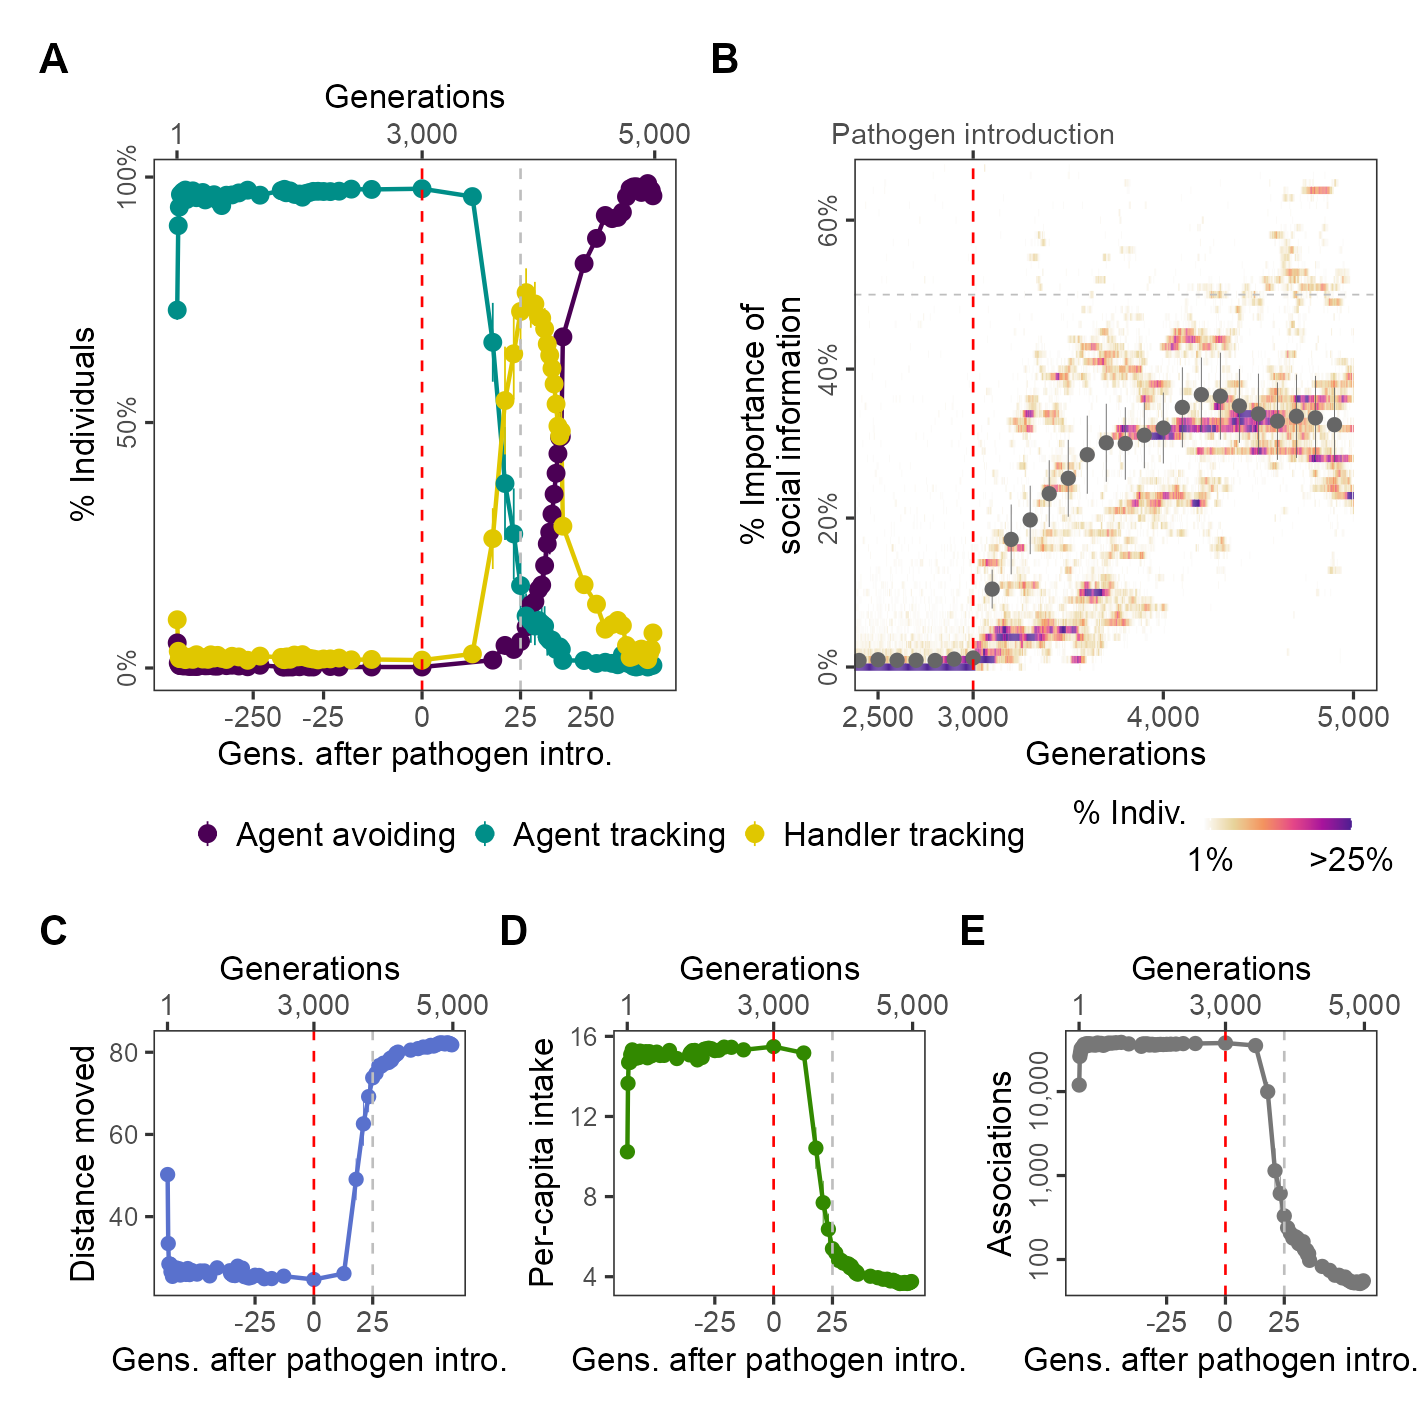
\includegraphics[width=8.7cm]{figures/fig_01.png}
% width=8.7cm,height=8.7cm
\caption{
    \textbf{Increased large-scale movement during natural molt, but reduced movement following manipulation in bulbuls and sparrows, but not reed warblers.}
    White-spectacled bulbuls (\textit{Pycnonotus xanthopygos}) and House sparrows (\textit{Passer domesticus}) moved $\approx$251\% and $\approx$150\% as far between areas of prolonged use (`residence patches') when molting, compared to non-molting individuals (generalised additive model estimates: bulbuls, $F$ = 4.734, p = 0.01; sparrows, $F$ = 11.58, p < 0.001).
    However, when bulbuls' and sparrows' wings were heavily compromised by experimental manipulation (wing gap index $\geq$ 12), both species made shorter movements between residence patches.
    In contrast, Clamorous reed warblers (\textit{Acrocephalus stentoreus}) did not show a significant difference in large-scale movements with increasing wing gap index, possibly because they are already restricted to small patches of reedbeds.
    Only statistically significant model fits are shown.
}\label{fig1}
\end{figure}

\begin{figure}[!t]
    \centering
    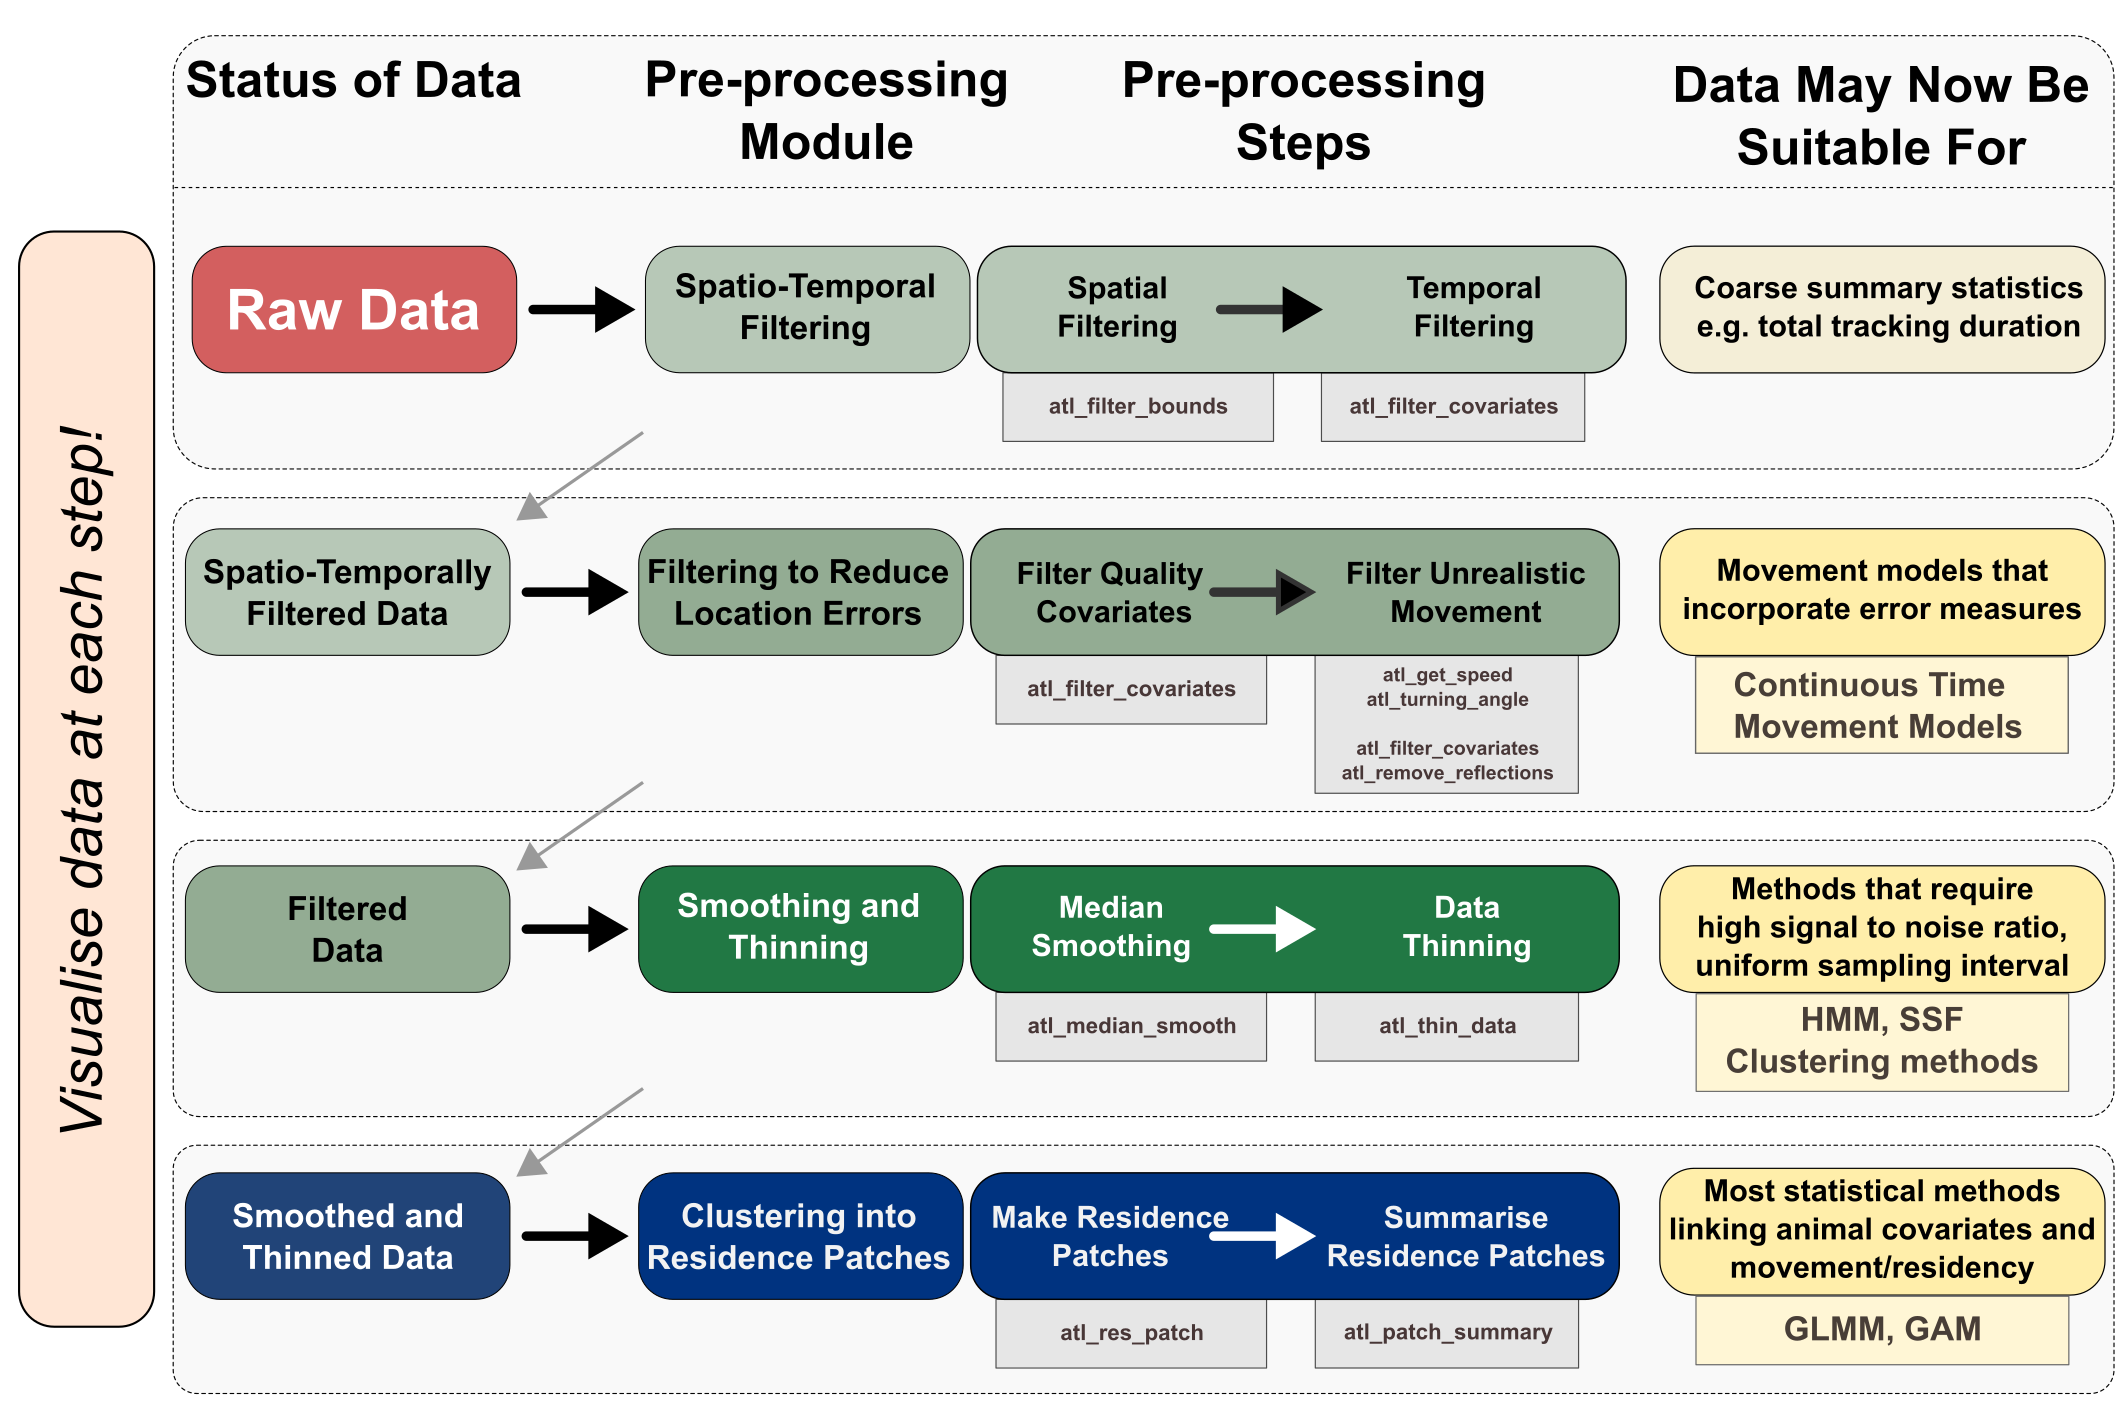
\includegraphics[width=8.7cm]{figures/fig_02.png}
    % width=8.7cm,height=8.7cm
    \caption{
        \textbf{Movement of slow-molting swallows is not affected by molt-related wing gaps.}
        Barn swallows (\textit{Hirundo rustica}) move about the same distance per hour (3.5 km) even while molting or artificially manipulated, as they do when they are not molting (generalised additive model estimate $F$ = 0.129, p = 0.723).
    }\label{fig2}
    \end{figure}

\subsection*{Birds select for sheltered viewsheds, regardless of molt status or vegetation}

To test whether flight feather molt affected birds' habitat selection, we examined whether wing gap size was associated with the visibility of individuals' residence patches.
Expecting that birds with larger wing gaps would have residence patches in more sheltered areas, we calculated the visibility index (a `fearscape') across our study area \cite{olsoy2015,aben2018,aben2021}.
The visibility index represents whether a location can be observed from surrounding areas, for example by a commonly occurring predator, the Eurasian sparrowhawk (\textit{Accipiter nisus}; see \textit{Methods}).
Areas with taller vegetation such as orchards, and built-up areas such as settlements have lower visibility indices and are more sheltered (see \textit{SI Appendix}), as predator lines of sight are obstructed by intervening objects \cite{olsoy2015}.
Though barn swallows hunt at low altitudes ($<$ 4m) and could use sheltering vegetation or structures \cite{warrick2016}, the ATLAS tracking system could not resolve individuals' altitude, and so we did not examine the use of shelter for swallows.

First, fitting a GAM with species-specific smooths for bulbuls, sparrows, and reed warblers (see \textit{Methods}), we found only a moderate overall relationship between the visibility index of residence patches and the size of the molt-related wing gap (GAM t-value = 100.5, p $<$ 0.001; $R^2$ = 0.312; Fig.~\ref{fig3}).
This suggests that birds select for sheltered areas of similar (low) visibility regardless of the size of their wing gap (visibility index, mean $\pm$ SD: bulbuls =  0.39 $\pm$ 0.18; sparrows = 0.47 $\pm$ 0.19; reed warblers = 0.38 $\pm$ 0.17).
Only reed warblers had slightly more sheltered patches with larger wing gaps (GAM estimate $F$ = 16.354, p < 0.001; Fig.~\ref{fig3}), potentially because their rapid molt rate severely reduces flight capacity and makes increased shelter necessary.

% Our results are consistent with most individuals' use of patches of natural vegetation (such as reedbeds) or semi-natural agriculture (such as orchards) in our landscape.
In our study area, shelter and vegetation productivity (proxied by NDVI; see \textit{Methods}) are correlated (GAM estimate $F$ = 172.49, p < 0.001), making it difficult to disentangle the sheltering effects of vegetation from its resource provisioning effects \cite{pettorelli2011}.
To account for this, we used a modified step-selection approach \cite{avgar2016,signer2019,aben2021}, to compare the visibility indices of individuals' residence patches, against the areas that these individuals could have used instead (see \textit{Methods}).
Fitting separate logistic regressions for each species and each broad molt status (non-molting, molting, and manipulated), we found that across molt status , all three species preferred low-visibility sites over higher visibility ones (Fig.~\ref{fig3}).
Furthermore, vegetation productivity was rarely a significant predictor of step-selection (see \textit{SI Appendix} Table {S1}).
This is consistent with the idea that birds avoid open agricultural fields, where they might be exposed to potential predators, even though fields are highly productive.

\begin{figure*}%[\sidecaptionrelwidth]
\centering
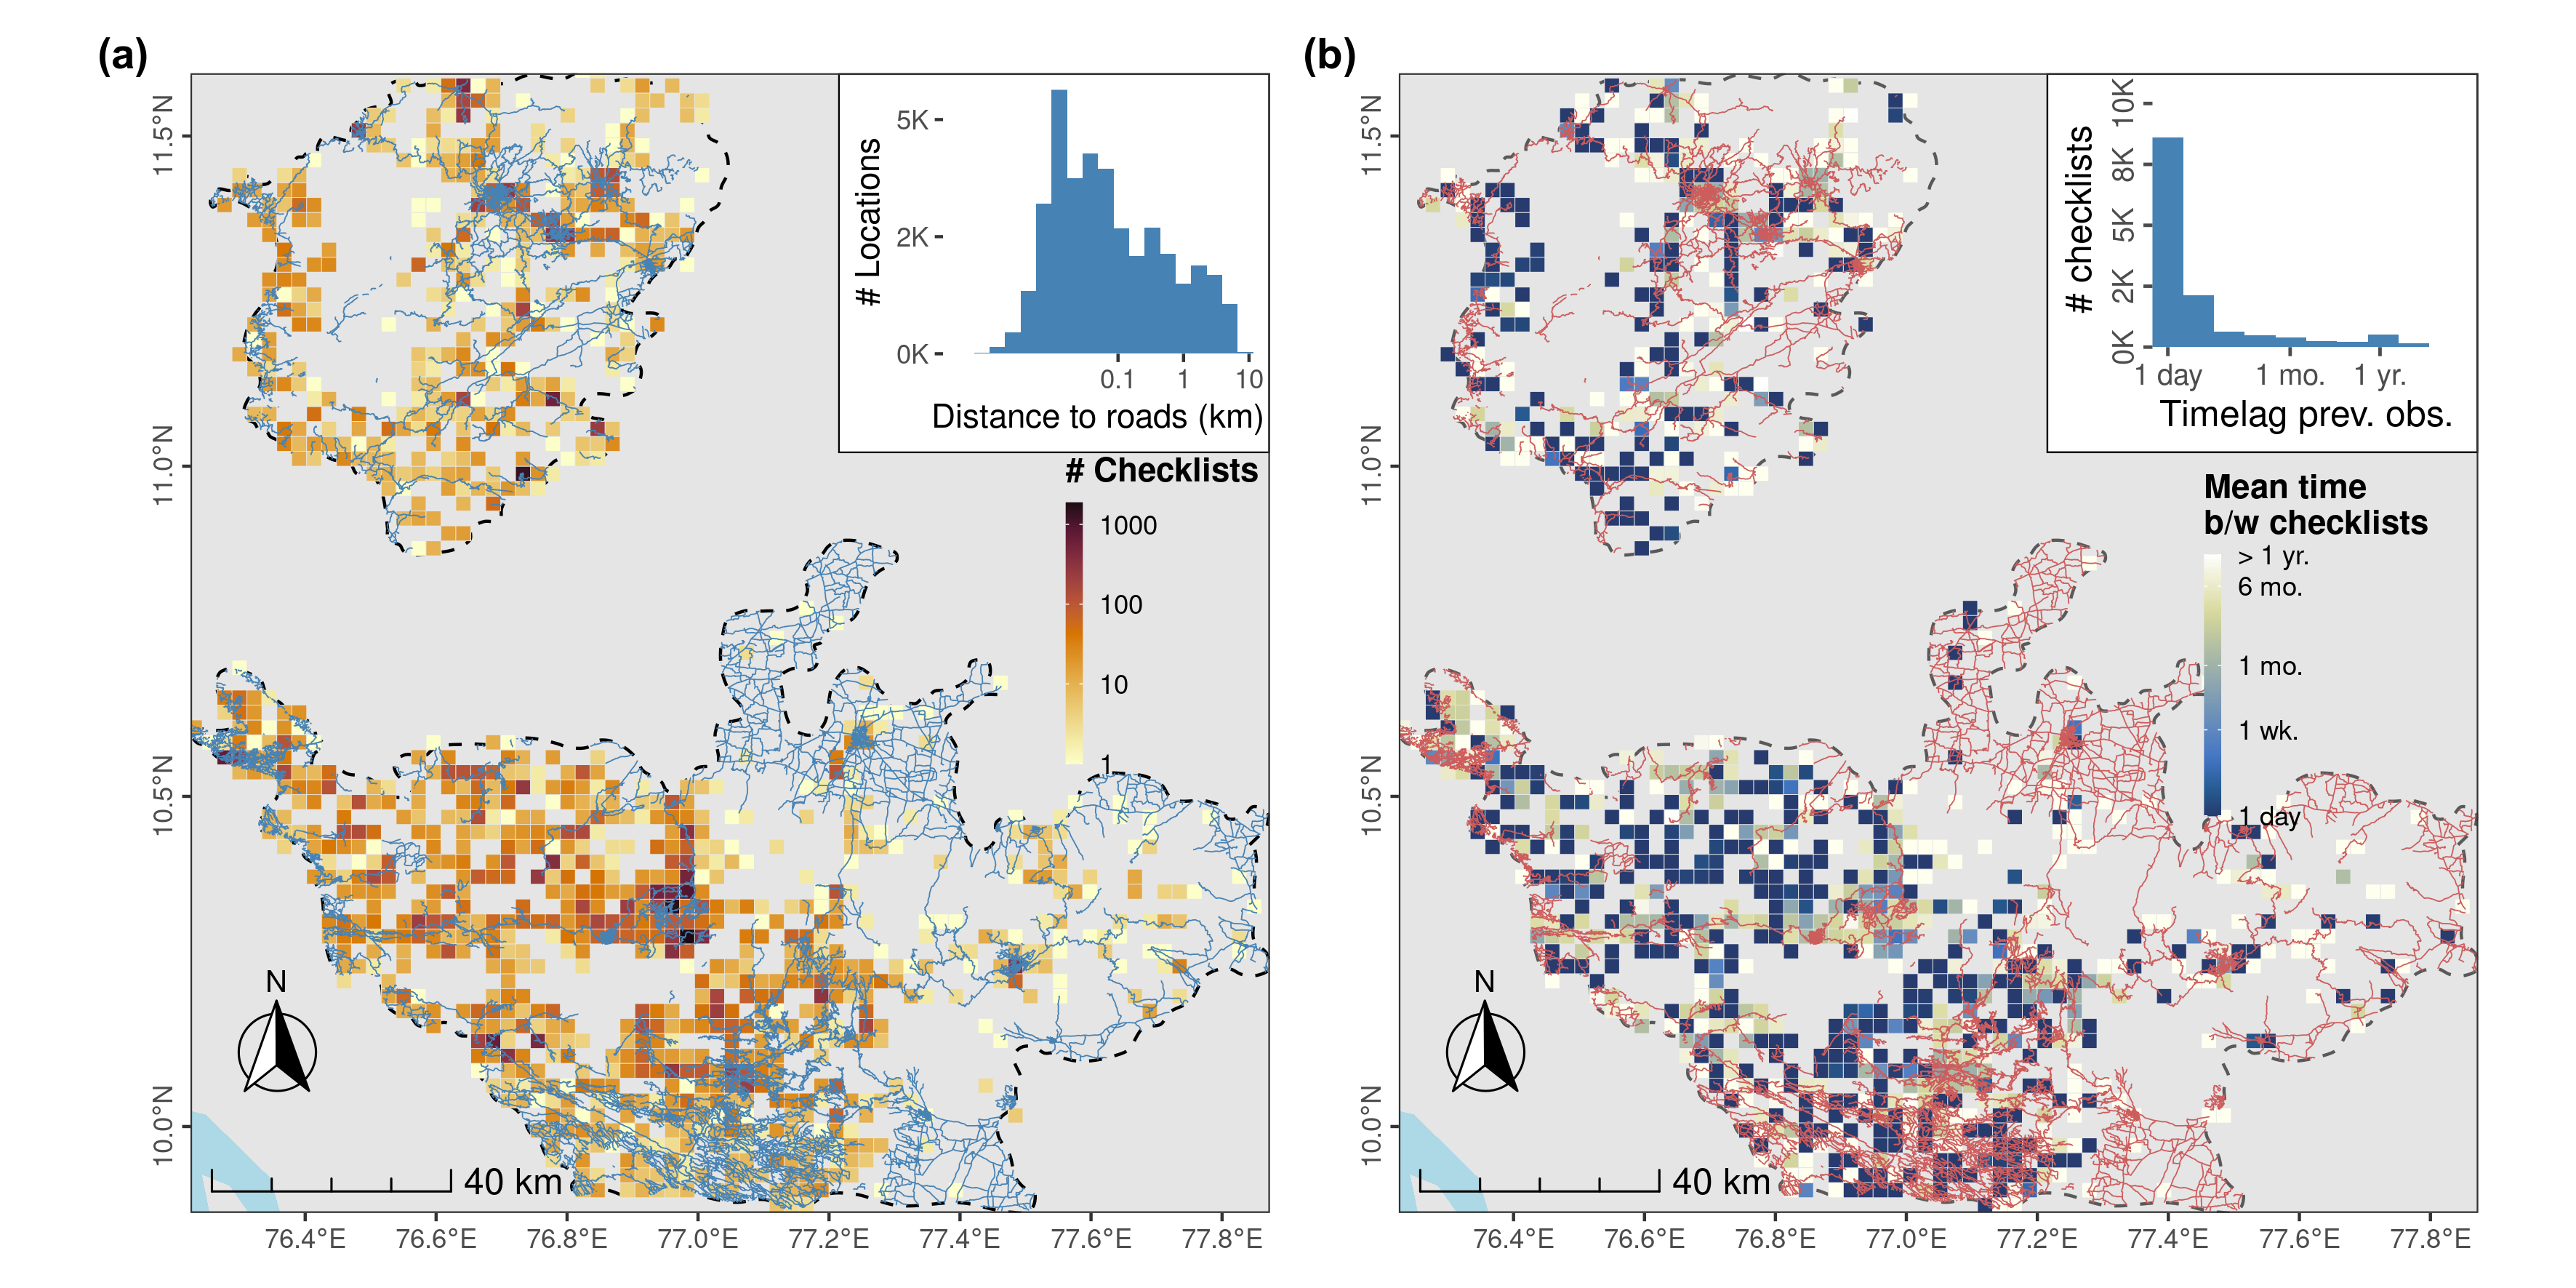
\includegraphics[width=17.8cm,height=8.7cm]{figures/fig_03.png}
% width=8.7cm,height=8.7cm
\caption{
    \textbf{Bulbuls, sparrows, and reed warblers prefer sheltered habitats across wing condition.}
    Across the three species, the molt-related wing gap index was a poor predictor of the visibility of areas actually occupied by individuals (`real' residence patches).
    Individuals' real residence patches were significantly more sheltered than nearby areas where individuals could have flown instead, indicating an active selection for sheltered, rather than simply vegetated areas.
    Step-selection coefficients for visibility are shown above average visibility index scores for real (circles) and potential residence patches (triangles).
    Coloured points represent raw visibility indices of real patches, while grey points in background show the much greater visibility indices of potential patches that individuals could have selected instead.
}\label{fig3}
\end{figure*}

\section*{Discussion}

Our study is among the first to quantify how the compromised wing surface associated with molt directly affects movement and habitat selection in wild birds.
Focusing on resident birds outside their breeding season, rather than migratory or breeding ones, enables at least some control on confounding factors associated with seasonal physiological changes, and the confounding effect of migration-related energy requirements \cite{alerstam1990,wikelski2003,horvitz2014}.
Both rapidly molting Clamorous reed warblers, and slow-molting Barn swallows, did not adjust their large-scale movements to their wing condition.
Reed warblers move very short distances ($<$ 25m) in low-visibility areas, and can afford rapid, resource-intensive feather regrowth \citep{lindstrom1993,newton2009,kiat2017}, as this does not compromise their ability to move scansorially through their reedbed habitat, which also offers shelter from predators.
At the other extreme, barn swallows which forage exclusively while flying have evolved a very slow molt rate \cite{kiat2016}, which likely prevents significant direct aerodynamic effects of feather loss on flight capacity.
Our work shows how birds' evolved molt strategies --- which are themselves influenced by movement strategies \cite{kiat2016} --- are interlinked with the direct, short-term effects of molt on movement.

We also show how birds with intermediate molt rates --- White-spectacled bulbuls and House sparrows --- can adapt their movement strategies to their wing condition.
Surprisingly, these species moved more when naturally molting than non-molting.
Birds can compensate for lower wing power output by growing their pectoral muscles, and this may allow them to maintain flight capacity during natural molt, enabling increased movement to find resources for feather growth \cite{chai1997,swaddle1997}.
However, increased movement for resources cannot compensate for the costs of inefficient flight and feather growth, moving less overall to conserve energy may be the optimal strategy until new flight feathers develop.
This latter strategy should be expected when the wing gap size is increased beyond the extent of natural molt, as in our study.
The shorter between-patch movements of artificially manipulated bulbuls and sparrows, compared with naturally molting birds, thus fit neatly within this framework.
Importantly, our relatively non-invasive method only increases the wing's feather gap size while avoiding wing injury, suggesting that the reduction in flight is actually due to considerations of flight efficiency, rather than trauma.

We have for the first time applied the idea of the cumulative viewshed to directly assess the availability of shelter from observation, along birds' real and potential movement paths \cite{olsoy2015}.
Birds, like other animals, are capable of taking the spatial perspective of other individuals \cite{emery2000,krams2001,watve2002,davidson2016}, i.e., whether a location would be visible to another observer, such as a predator \citep{watve2002,olsoy2015}.
Previous work has focused on demonstrating spatial perspective taking --- and resulting habitat selection --- at small spatial scales of a few metres, and typically with a direct predator cue \cite{krams2001,watve2002}.
Our work is the first to combine the spatial perspective-taking concept with the emerging framework of animal viewshed ecology at landscape scales \cite{aben2018,aben2021}.
We demonstrate that \textit{(i)} birds can estimate the visibility (and hence riskiness) of an area from multiple perspectives, \textit{(ii)} and that they can do so at relatively large, landscape scales (many dozens of metres).
Our results also show how the modelling of animal movement decisions should also incorporate individuals' estimates of what \textit{other animals} can see \cite{emery2000}.
Visibility analysis provides a simple, mechanistic way to incorporate animals' potential assessments of landscape risk into habitat selection models.
This could help move away from purely correlative studies of animal habitat selection, which usually rely on predictors with very broad applicability \cite{pettorelli2011}.

Our species strongly preferred sheltered, low-visibility habitats over more open sites, even when the available sites had similar vegetation productivity.
Predators are unlikely to always be in the vicinity of a specific location, or indeed to always be visible.
This instead point to a pre-emptive avoidance of open agricultural areas where predation risk is highest, showing the immediate, small-scale effects of a `fearscape' \cite{olsoy2015} on animal movement.
This pre-emptive caution may explain why wing condition, which should be expected to determine vulnerability to predation, did not lead to more sheltered residence patches in two of three species.
Furthermore, our work suggests that avoidance of high-visibility areas may be an overlooked mechanism by which agricultural `green deserts' exclude avian biodiversity, although the idea is applicable across taxa.
An unwillingness to break cover from sheltered areas, and move through high-visibility habitat, may explain how individual movement decisions can scale up to restrict animal space-use, from home-ranges to dispersal events \cite{schlagel2020}.
Overall, our work provides a template for combining simple experimental methods with technological advances in tracking technology, and with a mechanistic approach to landscape ecology, in the study of animal movement.

\section*{Acknowledgments}

This study was supported by the Minerva Center for Movement Ecology and the Minerva Foundation. 
P.R.G was supported by an Adaptive Life Programme grant made possible by the Groningen Institute for Evolutionary Life Sciences (GELIFES).
R.N. acknowledged support from the Adelina and Massimo Della Pergola Chair of Life Sciences.

\newrefcontext[sorting=nyt]
\section*{Literature Cited}
\printbibliography[title={Literature~Cited},heading=none]
\end{refsection}